\appendix
\section{Additional results}
\label{app:extra}

\subsection{Baseline details}
\label{app:baseline}
Table~\ref{tab:baseline} gives the baseline estimates on the development notes and Figure~\ref{fig:cgrid} the CV error across the $C$ grid. Errors are flat from $C=100$ to $C=1000$, so the baseline is effectively unregularised. The first rows of the cleaned data are in Table~\ref{tab:head}.

\begin{table}[H]
  \centering
  \caption{Logistic-regression baseline on the 1,078 development notes. SE is the standard error of the five fold errors. The 95\% interval is a Wilson interval on the pooled out-of-fold errors.}
  \label{tab:baseline}
  \small
  % generated by src/make_tables.py
\begin{tabular}{lrrl}
\toprule
Model / estimate & Error & SE & Notes \\
\midrule
Majority class & 45.3\% & -- & -- \\
Logistic regression, $C=100$ (5-fold CV) & 0.56\% & 0.09\% & 6/1078; 95\% CI 0.26\%--1.21\% \\
Logistic regression, nested 5$\times$5 CV & 0.74\% & 0.32\% & AUC 0.9999 \\
Logistic regression, 10 repeats of 5-fold & 0.54\% & -- & range 0.37\%--0.65\% \\
\bottomrule
\end{tabular}

\end{table}

\begin{table}[H]
  \centering
  \caption{First rows of the cleaned data, two per class.}
  \label{tab:head}
  \small
  % generated by src/make_tables.py
\begin{tabular}{rrrrc}
\toprule
Variance & Skewness & Kurtosis & Entropy & Class \\
\midrule
3.622 & 8.666 & -2.807 & -0.447 & 0 \\
4.546 & 8.167 & -2.459 & -1.462 & 0 \\
-1.397 & 3.319 & -1.393 & -1.995 & 1 \\
0.390 & -0.143 & -0.032 & 0.351 & 1 \\
\bottomrule
\end{tabular}

\end{table}

\begin{figure}[H]
  \centering
  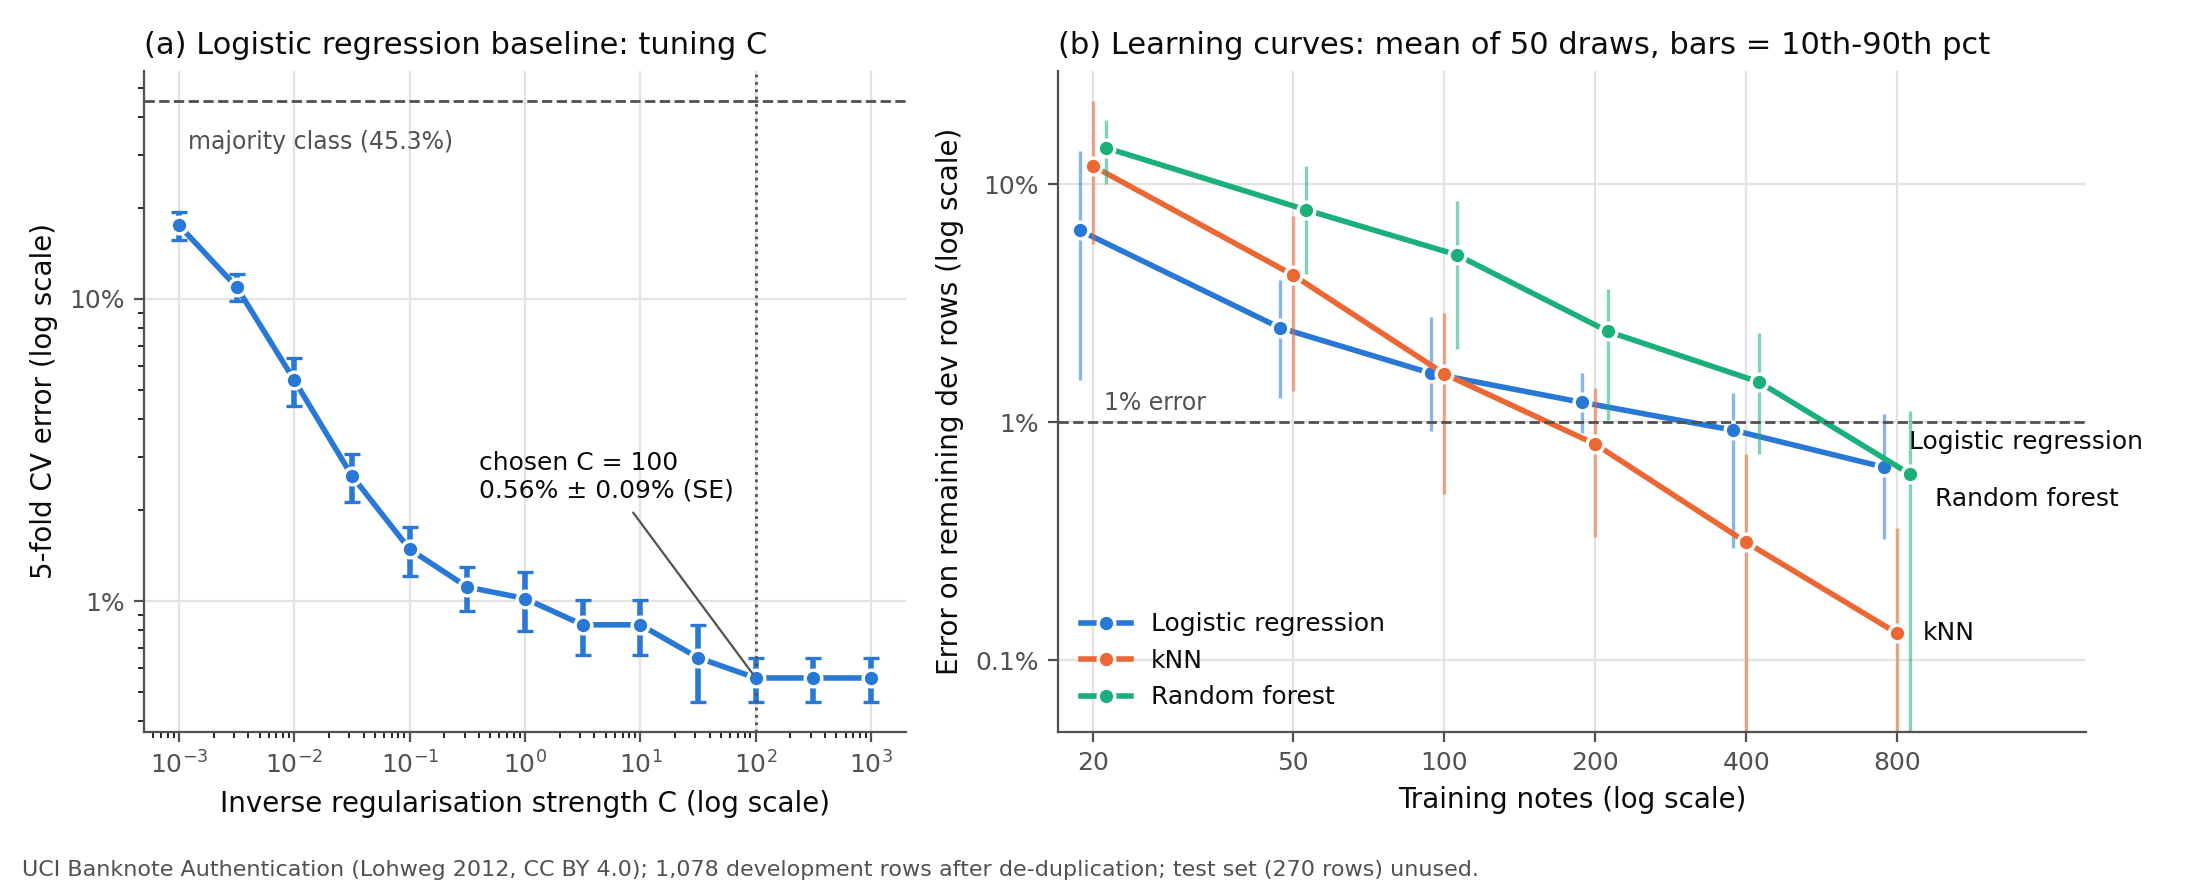
\includegraphics[width=\linewidth]{../figures/baseline.png}
  \caption{Baseline-checkpoint figure. (a) Logistic-regression CV error across the $C$ grid, $\pm$1 SE. (b) The first learning curves (three methods, six sizes); the main text extends these.}
  \label{fig:cgrid}
\end{figure}

\subsection{Full learning curves}
\label{app:full}
\begin{table}[H]
  \centering
  \caption{Mean error (\%) $\pm$ SE over 50 draws, scored on the development notes not used for training. Bold marks the lowest mean at each size. $^\dagger$Extension.}
  \label{tab:full}
  \small
  % generated by src/make_tables.py
\begin{tabular}{rccccc}
\toprule
$n$ & Logistic regression & $k$NN & Random forest$^\dagger$ & Gradient boosting$^\dagger$ & Neural network$^\dagger$ \\
\midrule
10 & 16.28 $\pm$ 1.51 & 21.57 $\pm$ 1.31 & 23.24 $\pm$ 1.47 & 21.00 $\pm$ 1.45 & \textbf{11.90 $\pm$ 1.41} \\
20 & 6.39 $\pm$ 0.85 & 11.89 $\pm$ 1.04 & 14.22 $\pm$ 0.71 & 15.68 $\pm$ 0.78 & \textbf{4.74 $\pm$ 0.51} \\
30 & 3.38 $\pm$ 0.33 & 7.11 $\pm$ 0.47 & 9.95 $\pm$ 0.52 & 11.70 $\pm$ 0.64 & \textbf{2.90 $\pm$ 0.34} \\
50 & 2.50 $\pm$ 0.20 & 4.15 $\pm$ 0.35 & 7.81 $\pm$ 0.45 & 8.92 $\pm$ 0.51 & \textbf{2.02 $\pm$ 0.20} \\
100 & 1.61 $\pm$ 0.11 & 1.60 $\pm$ 0.15 & 5.05 $\pm$ 0.34 & 5.34 $\pm$ 0.39 & \textbf{0.91 $\pm$ 0.10} \\
150 & 1.22 $\pm$ 0.07 & 0.99 $\pm$ 0.10 & 3.56 $\pm$ 0.23 & 3.13 $\pm$ 0.19 & \textbf{0.63 $\pm$ 0.08} \\
200 & 1.21 $\pm$ 0.06 & 0.81 $\pm$ 0.07 & 2.41 $\pm$ 0.15 & 1.91 $\pm$ 0.12 & \textbf{0.49 $\pm$ 0.06} \\
300 & 1.07 $\pm$ 0.06 & 0.56 $\pm$ 0.06 & 1.99 $\pm$ 0.12 & 1.88 $\pm$ 0.14 & \textbf{0.28 $\pm$ 0.05} \\
400 & 0.93 $\pm$ 0.05 & 0.31 $\pm$ 0.04 & 1.47 $\pm$ 0.09 & 1.17 $\pm$ 0.08 & \textbf{0.12 $\pm$ 0.03} \\
600 & 0.82 $\pm$ 0.06 & 0.13 $\pm$ 0.03 & 1.05 $\pm$ 0.07 & 0.66 $\pm$ 0.07 & \textbf{0.06 $\pm$ 0.02} \\
800 & 0.65 $\pm$ 0.06 & 0.13 $\pm$ 0.03 & 0.60 $\pm$ 0.06 & 0.33 $\pm$ 0.06 & \textbf{0.00 $\pm$ 0.00} \\
\bottomrule
\end{tabular}

\end{table}

\begin{table}[H]
  \centering
  \caption{Paired difference from logistic regression, in percentage points (negative is better than the baseline), with the number of draws (out of 50) in which the method beat / lost to the baseline; the rest are ties. Bold: $|\Delta|>2$ SE.}
  \label{tab:paired}
  \small
  \resizebox{\linewidth}{!}{% generated by src/make_tables.py
\begin{tabular}{lccccccc}
\toprule
$n$ & 10 & 20 & 50 & 100 & 200 & 400 & 800 \\
\midrule
$k$NN & \textbf{+5.28} (16/34) & \textbf{+5.50} (9/40) & \textbf{+1.66} (14/35) & $-$0.01 (27/19) & \textbf{$-$0.40} (37/9) & \textbf{$-$0.61} (45/0) & \textbf{$-$0.52} (41/2) \\
Random forest$^\dagger$ & \textbf{+6.96} (13/37) & \textbf{+7.83} (5/45) & \textbf{+5.31} (1/49) & \textbf{+3.44} (1/49) & \textbf{+1.19} (8/41) & \textbf{+0.55} (7/37) & $-$0.04 (21/20) \\
Gradient boosting$^\dagger$ & \textbf{+4.72} (18/32) & \textbf{+9.29} (6/44) & \textbf{+6.43} (1/49) & \textbf{+3.74} (0/50) & \textbf{+0.69} (12/34) & \textbf{+0.24} (15/30) & \textbf{$-$0.32} (34/9) \\
Neural network$^\dagger$ & \textbf{$-$4.39} (33/16) & \textbf{$-$1.65} (29/18) & \textbf{$-$0.47} (31/14) & \textbf{$-$0.70} (44/2) & \textbf{$-$0.72} (47/1) & \textbf{$-$0.81} (50/0) & \textbf{$-$0.65} (45/0) \\
\bottomrule
\end{tabular}
}
\end{table}

\begin{table}[H]
  \centering
  \caption{Most common hyperparameters chosen by inner CV, with the share of the 50 draws that chose them. For the forest, $m$ is the number of features tried per split.}
  \label{tab:params}
  \small
  \resizebox{\linewidth}{!}{% generated by src/make_tables.py
\begin{tabular}{lllll}
\toprule
Method & $n=10$ & $n=50$ & $n=200$ & $n=800$ \\
\midrule
Logistic regression & $C=0.001$ (38\%) & $C=3.16$ (30\%) & $C=1$ (26\%) & $C=100$ (42\%) \\
$k$NN & $k=1$ (80\%) & $k=1$ (68\%) & $k=1$ (80\%) & $k=1$ (98\%) \\
Random forest$^\dagger$ & $m=1$, leaf 1 (60\%) & $m=1$, leaf 1 (56\%) & $m=1$, leaf 1 (66\%) & $m=1$, leaf 1 (52\%) \\
Gradient boosting$^\dagger$ & $\eta=0.05$, depth 1 (84\%) & $\eta=0.05$, depth 1 (52\%) & $\eta=0.2$, depth 1 (50\%) & $\eta=0.2$, depth 3 (86\%) \\
Neural network$^\dagger$ & 8 units, $\alpha=0.0001$ (54\%) & 8 units, $\alpha=0.0001$ (50\%) & 8 units, $\alpha=0.0001$ (44\%) & 8 units, $\alpha=0.0001$ (72\%) \\
\bottomrule
\end{tabular}
}
\end{table}

\subsection{Grouped draws}
\label{app:grouped}
\begin{table}[H]
  \centering
  \caption{Mean error (\%) $\pm$ SE for random draws and for draws that keep each 8-row pseudo-specimen on one side of the split (training, inner CV folds and evaluation).}
  \label{tab:grouped}
  \small
  % generated by src/make_tables.py
\begin{tabular}{rcccc}
\toprule
 & \multicolumn{2}{c}{Logistic regression} & \multicolumn{2}{c}{$k$NN} \\
\cmidrule(lr){2-3}\cmidrule(lr){4-5}
$n$ & random & grouped & random & grouped \\
\midrule
50 & 2.50 $\pm$ 0.20 & 2.30 $\pm$ 0.28 & 4.15 $\pm$ 0.35 & 4.53 $\pm$ 0.44 \\
100 & 1.61 $\pm$ 0.11 & 1.86 $\pm$ 0.17 & 1.60 $\pm$ 0.15 & 1.57 $\pm$ 0.18 \\
200 & 1.21 $\pm$ 0.06 & 1.14 $\pm$ 0.04 & 0.81 $\pm$ 0.07 & 0.74 $\pm$ 0.06 \\
400 & 0.93 $\pm$ 0.05 & 0.96 $\pm$ 0.06 & 0.31 $\pm$ 0.04 & 0.30 $\pm$ 0.05 \\
800 & 0.65 $\pm$ 0.06 & 0.71 $\pm$ 0.08 & 0.13 $\pm$ 0.03 & 0.13 $\pm$ 0.03 \\
\bottomrule
\end{tabular}

\end{table}

\subsection{Random-forest tuning}
\label{app:forest}
\begin{table}[H]
  \centering
  \caption{Random forest on all development notes. Top: 5-fold CV error of the small grid used inside every draw against a 64-setting grid. Bottom: out-of-bag error against the number of trees ($m=2$).}
  \label{tab:forest}
  \small
  % generated by src/make_tables.py
\begin{tabular}{lrcl}
\toprule
Grid & Configs & CV error (\%) & Best setting \\
\midrule
small (used in curves) & 6 & 0.56 $\pm$ 0.27 & $m=2$, leaf 1, 200 trees \\
large & 64 & 0.46 $\pm$ 0.21 & $m=3$, leaf 1, 500 trees, gini \\
\bottomrule
\end{tabular}

\vspace{4pt}
\begin{tabular}{lrrrrrr}
\toprule
Trees & 25 & 50 & 100 & 200 & 500 & 1000 \\
\midrule
OOB error (\%) & 0.74 & 0.56 & 0.46 & 0.56 & 0.65 & 0.74 \\
\bottomrule
\end{tabular}

\end{table}

\subsection{Test-set ROC curves}
\label{app:roc}
\begin{figure}[H]
  \centering
  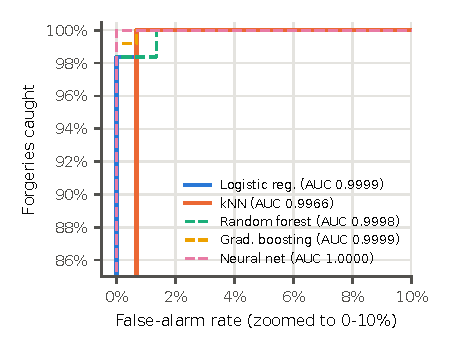
\includegraphics[width=0.55\linewidth]{../figures/test_roc.pdf}
  \caption{ROC curves on the 270 test notes, zoomed to the top-left corner.}
  \label{fig:roc}
\end{figure}

\section{Reproducibility}
\label{app:repro}
All code, the fixed split and the result files are at \url{https://github.com/maanasgoel/ese5420-banknote}. \texttt{src/baseline.py}, \texttt{src/learning\_curves.py}, \texttt{src/analyse.py} and \texttt{src/test\_eval.py} produce every number, and \texttt{src/make\_tables.py} writes every table and every number quoted in the text, so the paper cannot drift from the results. The full run takes about 20 minutes on an 8-core laptop (Python 3.10, scikit-learn 1.7.2).
